\documentclass[main.tex]{subfiles}


\begin{document}

\section{Supplementary Figures}
\label{suppfigs}


\begin{suppfigure}[H]
	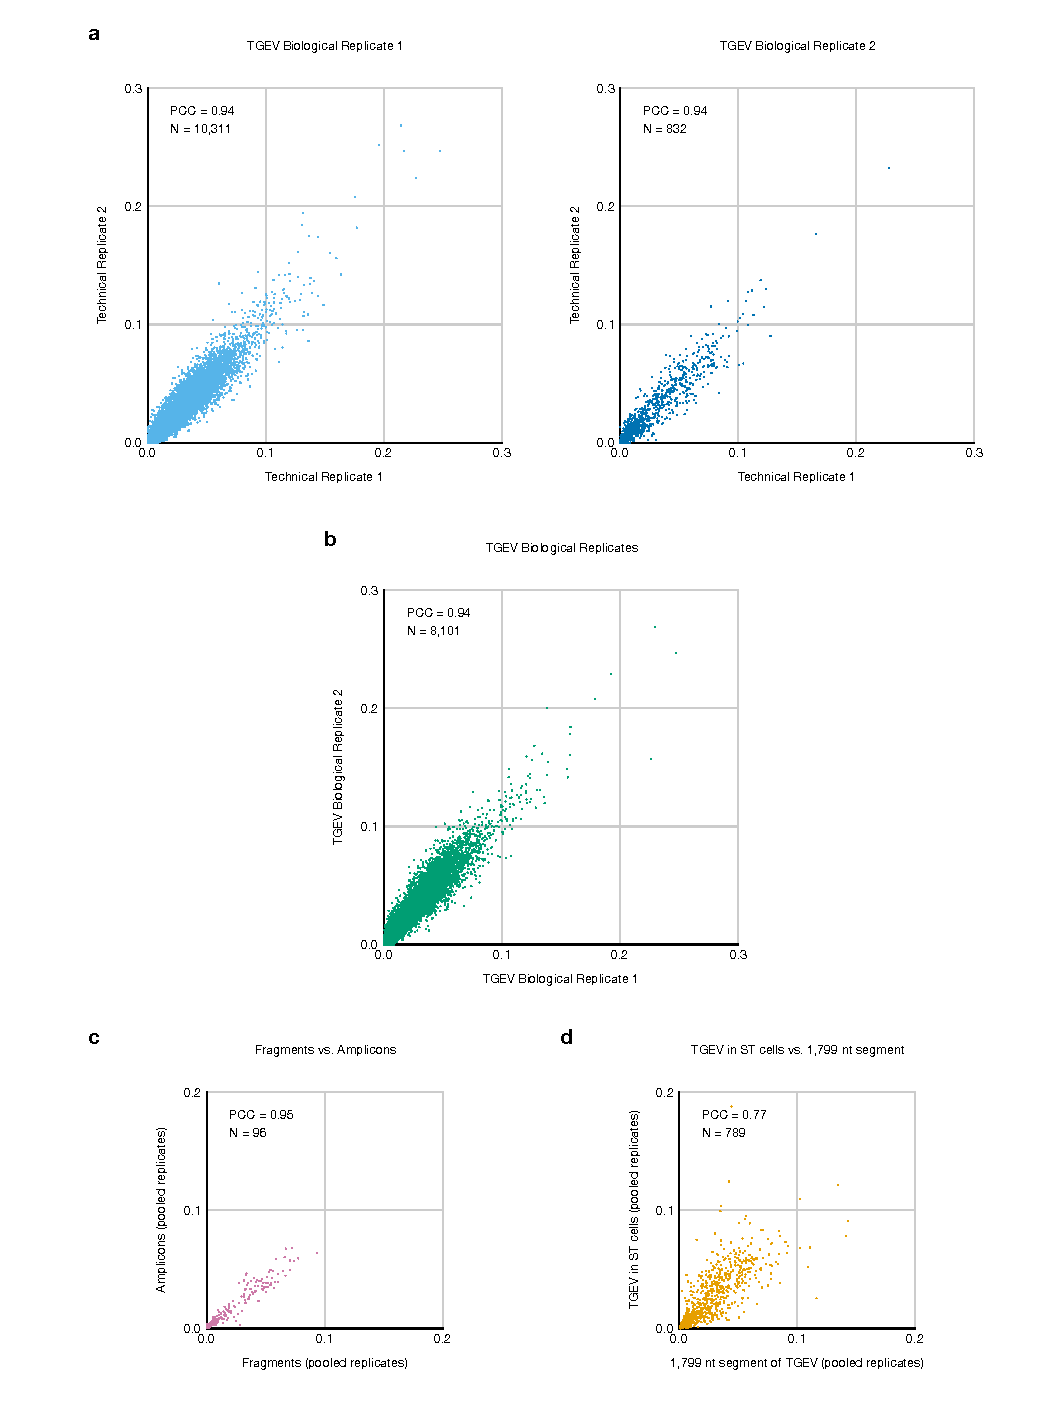
\includegraphics[width=\textwidth]{../SupplementaryFigures/tgev_reps.pdf}
	\caption{\textbf{Replicates of TGEV in ST cells and comparison to the 1,799 nt segment.} \textbf{(a)} Scatter plots comparing the DMS reactivities of the two technical replicates for each biological replicate of TGEV in ST cells. Each point represents one base in the sequence. The number of points (N) and Pearson correlation coefficient (PCC) are indicated for each plot. \textbf{(b)} Scatter plot comparing the DMS reactivities of the two biological replicates (each biological replicate comprises the reads for both of its technical replicates pooled together). \textbf{(c)} Scatter plot comparing the DMS reactivities of TGEV in ST cells (the reads for both biological replicates pooled together) and for the 1,799 nt segment \textit{in vitro}.}
	\label{tgev_reps}
\end{suppfigure}


\begin{suppfigure}[H]
	\includegraphics[width=\textwidth]{../SupplementaryFigures/tgev_5utr.pdf}
	\caption{\textbf{Secondary structure of the 5' UTR of transmissible gastroenteritis virus.} \textbf{(a)} Model of the secondary structure of the first 520 nt of the TGEV genome, based on DMS reactivities in infected ST cells. Bases are colored by DMS reactivity. The model includes the highly conserved stem loops SL1, SL2, SL4, SL5a, SL5b, and SL5c, as well as the more variable stem loops SL3, SL6, SL7, and SL8~\cite{Yang2015a}. The leader transcription regulatory sequence (TRS-L)~\cite{Alonso2002}, upstream open reading frame (uORF)~\cite{Nakagawa2016}, and start codon of ORF1 are also labeled. The model was drawn using VARNA~\cite{Darty2009}. \textbf{(b)} Receiver operating characteristic curve showing agreement between the DMS reactivities and the secondary structure model; the area under the curve (AUC) is indicated.}
	\label{tgev_5utr}
\end{suppfigure}



\end{document}
